\section{Background}
A sequential decision-making problem can be formulated as a Markov Decision Process (MDP) with Markov property satisfied. In an MDP, we have a set of \textit{states} $S$, a set of \textit{actions} $A$ and a policy space $\Pi$. An agent follows a \textit{policy} $\pi: S \rightarrow A$ that determines which action to take in a given state to interact with the environment $\xi$. After taking action $a$ in state $s$, the environment responds with some immediate loss $L$ and takes the agent to the next state $s'$ according to the transition probability $T(s'|s,a)$. We denote $d_\pi^t$ the state distribution at time $t$ after executing $\pi$ from time 1 to $t-1$, then the $T$-step expected loss of $\pi$ is $J(\pi) = \sum_{t=1}^T \mathbb{E}_{s'\sim d_\pi^t} \big[L(s, \pi(s)\big]  $.  Our goal is to learn a policy that minimize the task loss $J(\pi)$. Since in our problem we conduct an action at a time, the task is partially observed. We therefore consider the sequences of actions and observations, $s_t = x_1, a_1, x_2, a_2, ..., a_{t-1}, x_t$, and learn a strategy based on these sequences. Given a maximum number of actions that the agents can take, this formulation is a large finite state MDP. We can use reinforcement learning methods for MDPs. In this paper we employ an imitation learning approach.

In imitation learning, we define an oracle that executes policy $\pi^*$ and demonstrates action $a_s^* = \arg \min_{a\in A} C(s,a)$ in state $s$, where $C(s,a)$ is the oracles measure of the quality of $a$ given $s$. We use the Q-value of the state-action pair as $C(s,a)$ in this paper. The learner attempts to imitates the oracle's behavior without notion of the task loss function. Thus minimizing the task loss is reduced to minimizing a \textit{surrogate loss} with respect to the oracle's policy.

\section{Approach}

Our framework is shown in Figure~\ref{fig:flowchart}. Given an image and a query class, our algorithm detects the query class of objects by sequentially making decision of exploring one context/object class at a time, and narrow down the search area for the query based on observed responses. Our goal is to learn a policy $\pi(s)$ that can dynamically selects different sequences of ``questions''  given different query classes and images. We model the problem as an MDP and use reinforcement learning, specifically imitation learning to learn class-specific policy. 

%Under certain budget constraint, our goal is to learn a policy $\pi(s)$ that can sequentially select a contextual object class to detect  to narrow down the search area of the query or make an early rejection.  \HHNote{not sure what episode means hear..}of selecting actions for the input image $X$ and target query class $c_q$ \HHNote{$X$ and $c_q$ are not used here and they will be defined in the next section. Consider removing the notations}.

\begin{figure*}[htb]
\begin{center}
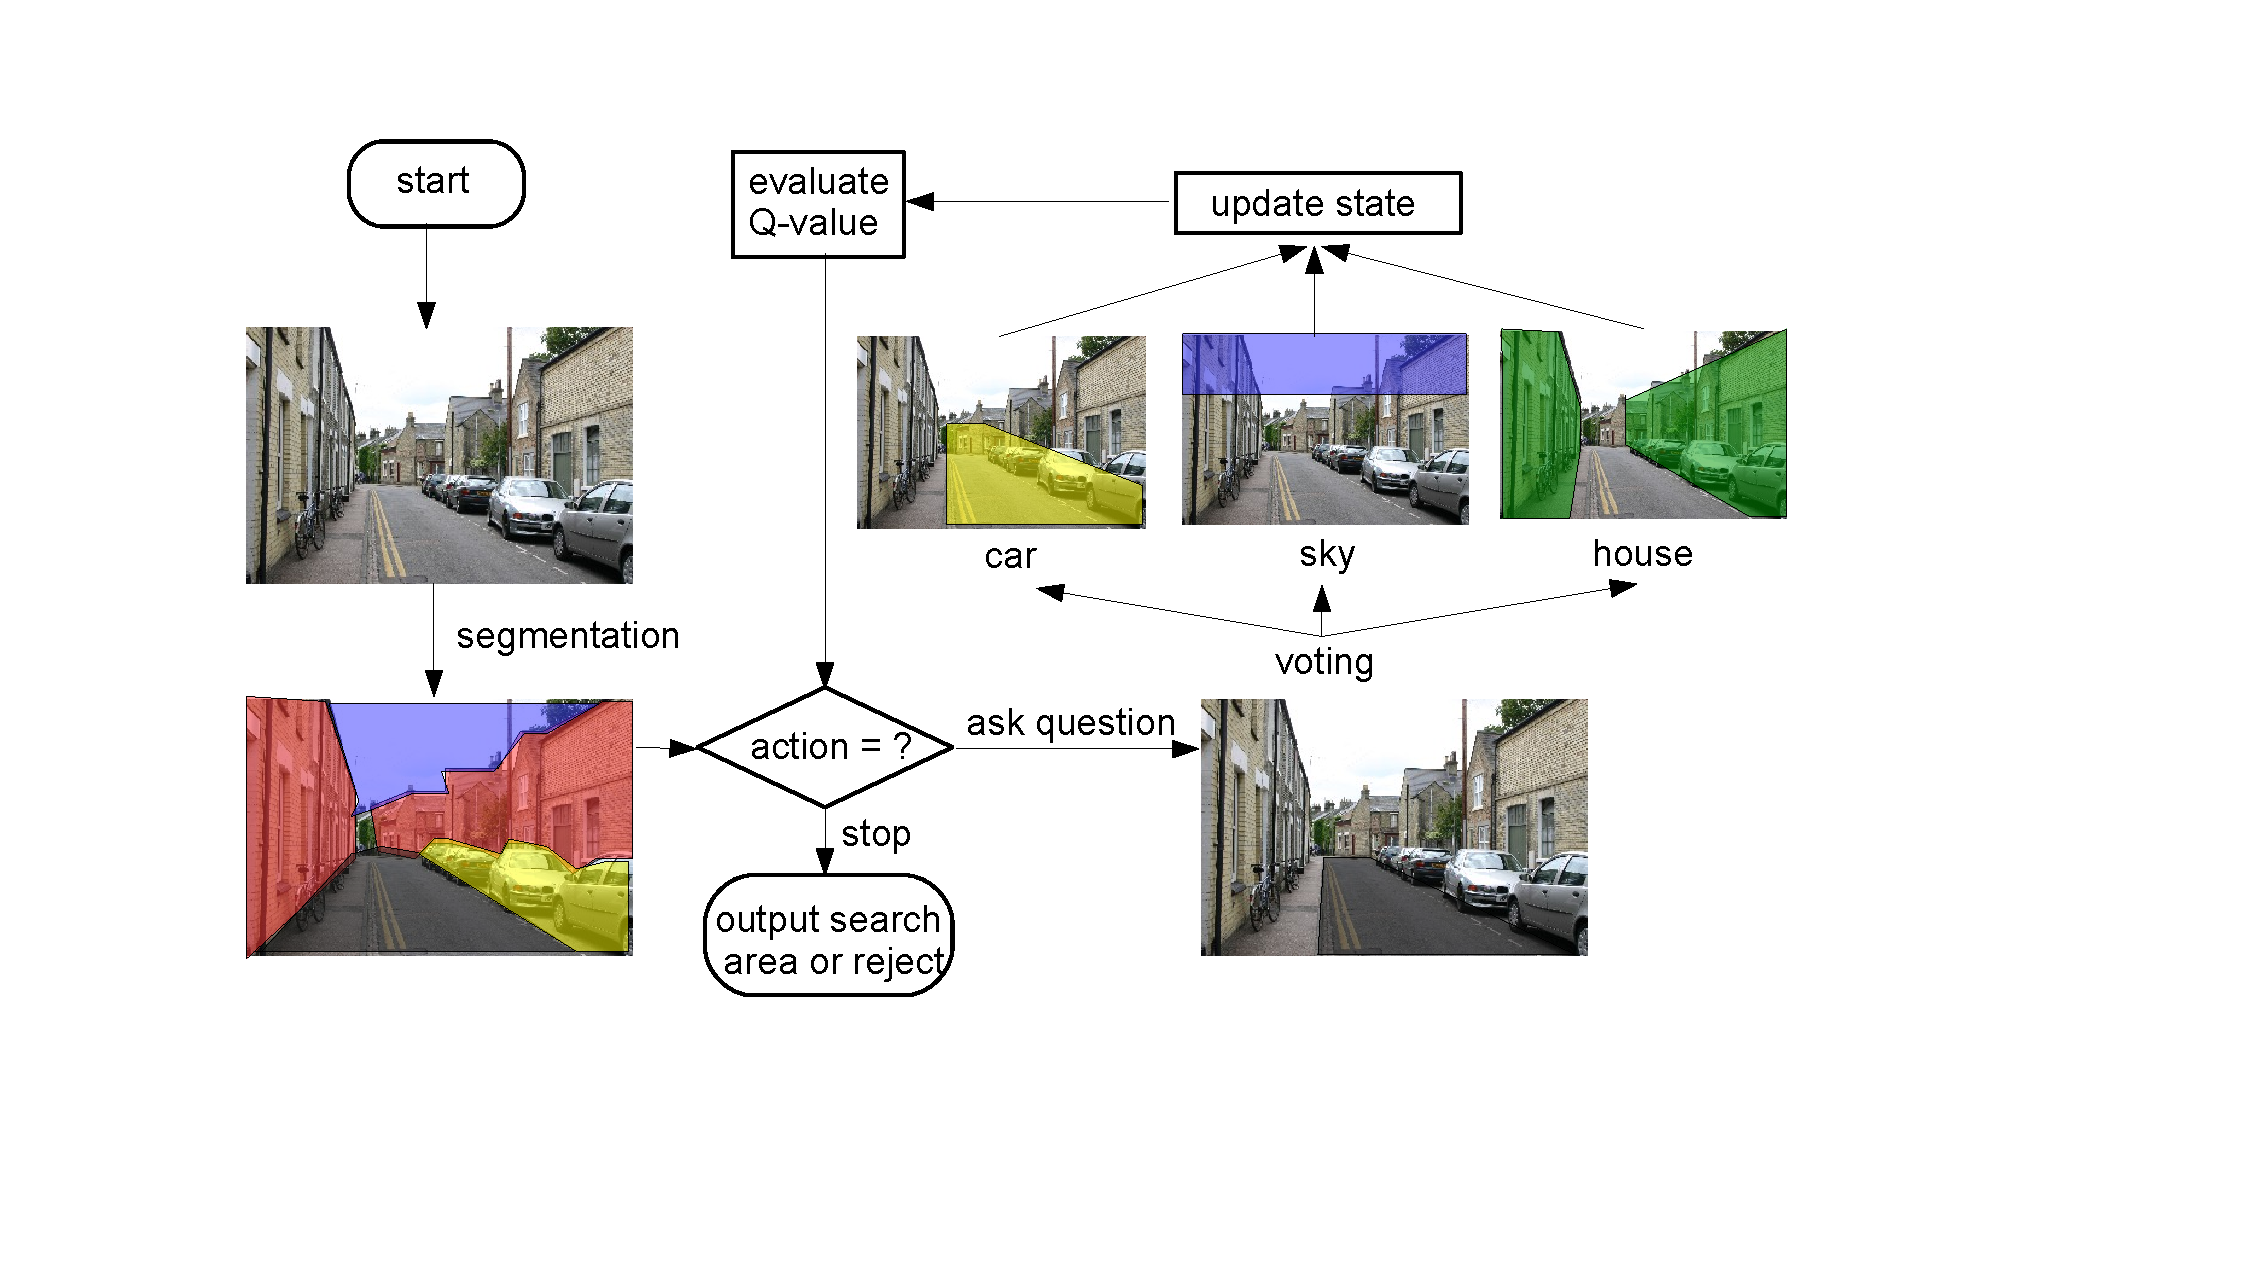
\includegraphics[width=\linewidth]{figures/flowchart_Q.pdf}
\caption{Framework of our context driven object searching. We first generate region hypotheses using object proposal algorithms, then the policy evaluates the current state and iteratively selects the action maximizing the Q-value function. Afterwards, the possible search locations are updated and the posterior probabilities of each category are evaluated for the next state.}
\label{fig:flowchart}
\end{center}

\end{figure*}

\subsection{Object Detection as Markov Decision Process (MDP)}
\label{sec:policy}

Specifically, given an image $X$ and a query object class $c_q$ in classes ${1,..,C}$, we define the MDP as follows.
\begin{mydef}
 The \textbf{detection action selection MDP} is defined by the tuple $(\mathcal{S}, \mathcal{A}, T(.), R(.), \gamma)$:
\begin{itemize}
\item \textbf{State} $s(t) = (X, O^t)\in \mathcal{S}$ that includes the image $X$ and the observations $O^t= \{x_1, x_2, ....,x_t\}$ over time till $t$. %  \HHNote{I would give some explanation of what state is before the math, e.g. a state contains necessary information for decision making}
\item The set of \textbf{actions} to be taken in each state $\mathcal{A} = \{a_1, ..., a_C, \mbox{Stop}, \mbox{Reject}\} $, where $a_i$ is to run the detector of class $c_i$, \textit{Reject} to reject query class in the image and terminate the process, and \textit{Stop} to output the search area and run query detector.
\item \textbf{State transition} function $T(s'|s,a, X)$ is the probability taking the agent to the next state $s'$ from $s$ by action $a$, depending on the instance $X$
\item The \textbf{reward} function $R(s,a,s') \rightarrow \mathbb{R}$ gives reward to taking action $a$ at state $s$ to the next state $s'$
\item The \textbf{discount} constant $\gamma$ defines a tradeoff between taking the action by greedily maximizing the immediate reward or the considering the long term expected reward.
\item The \textbf{policy} $\pi(s): \mathcal{S} \rightarrow \mathcal{A}$ is a mapping from a state to an action.
\end{itemize}
\end{mydef}

During test time, our search policy  iteratively selects an action $a^t \in \mathcal{A}$. Then the policy obtains response $x_t$ at time step $t$ given by the detection or classification results of action $a_t$. 

\HHNote{The causal relation ``since ... we want ... then define a policy'' here doesn't seem to be right. Policy and Q-value are defined by the MDP.} 
Formally, since we would like to select the actions dynamically, we want to learn a value function taking action $a$ in state $s$ under the policy $\pi$, denoted $Q^\pi(s,a): S\times A \rightarrow \mathbb{R}$, where $S$ is the space of all possible states, to assign a value to a potential action $a\in A$ given the current state. We can then define policy $\pi$ to take the action that maximizes the expected value:

\begin{eqnarray}
\label{eq:pi}
\pi(s) = \arg\max_{a_i\in A\backslash R} Q(s,a_i)
\end{eqnarray}

\subsection{Reward Function}

We define the \textit{immediate reward} $R$ as the immediate gain in intersection/union of the search space after conducting action $a_i$ at time step $t$ under state $s$ as:

\begin{eqnarray}
\label{eq:imreward}
R(s^t,a_i) =  \frac{X^{t+1}_i \cap X_q}{X^{t+1}_i \cup X_q} - \frac{X^{t}_i \cap X_q}{X^{t}_i \cup X_q}
\end{eqnarray}
where $X^{t+1}_i$ is the updated search area after executing action $a_i$ in state $s_t$, determined by the context models described in Section~\ref{sec:context}. $X_q$ is the groundtruth mask of the query object instances in the image. 
  
%at each time step $t$, we select a question $q_t$ and take action $a_t$ to evaluate it. Let $R^t = \{r_1, r_2, ....,r_t\}$ be the observations of responses to the actions taken at time $1...t$, where the response $r_t = p(c_t|X)$ is the detection or classification probability of class $c_t$ corresponding to question $q_t$. 




\subsection{Imitation Learning of Policy}
We propose a policy to use maximum expected reward to select $a_t$. To learn such a policy, we adopt a standard Q-learning algorithm~\cite{barto1998reinforcement}, where the action-value function is estimated by the Bellman equation recursively:
\begin{eqnarray}
\label{eq:bellman}
Q^*(s,a) = \mathbb{E}_{s'\sim \xi} \big[ R + \gamma \max_{a'} Q^*(s',a')|s,a \big]
\end{eqnarray}
where $a'$ and $s'\in\xi$ is the possible action-state pairs at the next time steps $t+1$.

Since the space of possible states $S$ is continuous and intractable, we use a linear approximation of the $Q$-values:
\begin{eqnarray}
\label{eq:qvalue}
Q^{\pi}(s,a) = \theta_\pi^T \phi(s,a) 
\end{eqnarray}

where $\phi(s,a) = \phi((X, O^t),a) = \phi(X^t,a)$ is the feature of the underlying area $X^t$ at time $t$ after observing detector responses of $a_1,...,a_t$. 

The parameters $\theta_\pi$ are learned by \textit{policy iteration}. We collect $(s,a,r,s')$ samples by running episodes starting from a random or empty state, then we search and prune in the tree of states and collect states samples  and corresponding features. To prevent overfitting, an $L_2$ regularized regression is trained for each class to predict the Q-values given current states.

\subsection{Context Modeling}
\label{sec:context}
Since our task is not only to detect the object but also refine the search space of the query in the image as accurately as possible, conventional modeling of context as simple co-occurrence statistics is inadequate. Instead we present a data-driven location aware approach to represent the spatial correlation between the objects and the scene. 

Here we formulate the context $p(c_t|c,X)$ as a posterior of the probabilistic vote map $p(c|c_t,X_s)$ defined on each pixel $(x_i,x_j)\in X$ over the image, and the responses of class $c_t$ after action $a_t$:
\begin{eqnarray}
p(c_t|c,X) = \sum_{s\in X^t} p(c|c_t,X_s)p(c_t|X_s)
\end{eqnarray}

Given a refined search space $X^t\in X$ of a context class $c_t$ at time $t$, we formalize $p(c|c_t,X)$ as a weighted vote from the cooccurring region pairs of class $c_t$ and $c$ in training scenes. Let $(s_{c_t}^i, s_c^i)$ be the $i$-th pair of co-occurring regions of class $c_t$ and $c$, and $b_{c_t}^i$ and $b_c^i$ be the corresponding bounding boxes. We can now define the probabilistic vote map $p(c|c_t,X)$ as:
\begin{eqnarray}
\label{eq:votemap}
p(c|c_t,X_s)_{s\in X^t} = \frac{1}{Z_c}\sum_i W(s_{c_t}^i,s;\theta^W).T(b_{c_t}^i,b_c^i)
\end{eqnarray}
where $s\in X^t$ is a region within the search space of the context class $c_t$. $Z_c$ is the normalization function. $W(.)$ is a kernel measuring similarity of region $s$ with a training region $s_i$. $T(b_{c_t}^i,b_c^i)$ models the transformation from $b_{c_t}^i$ to $b_c^i$, including translation and scaling. Figure~\ref{fig:votemap} shows a few examples of the vote maps. We can see that with the exemplar based and semantically aware voting, the resulted vote maps give more accurate search area of the query objects.


\begin{figure}[ht!]
\begin{center}
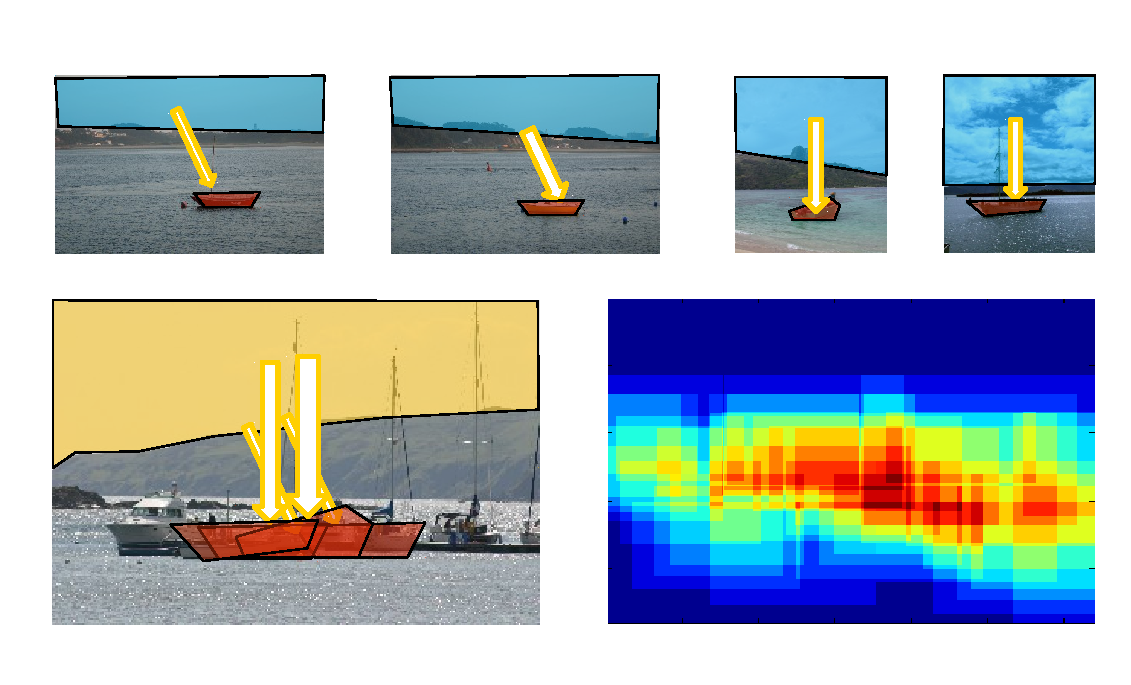
\includegraphics[width=0.6\linewidth]{figures/vote_sky_boat.pdf}
\end{center}
\caption{Examples of our weighted vote map for the context from sky to boat. The first rows are the training sample pairs of sky and boat and the second row is the test image and the resulted weighted voting map. The widths of the arrows denote the weighted similarity $W(s_{c_t}^i,s;\theta^W)$ between the test segment of sky (highlighted in yellow) and a training instance of sky segment (in light blue)}
\label{fig:vote_sky_boat}
\end{figure}


\begin{figure}[ht!]
\begin{center}
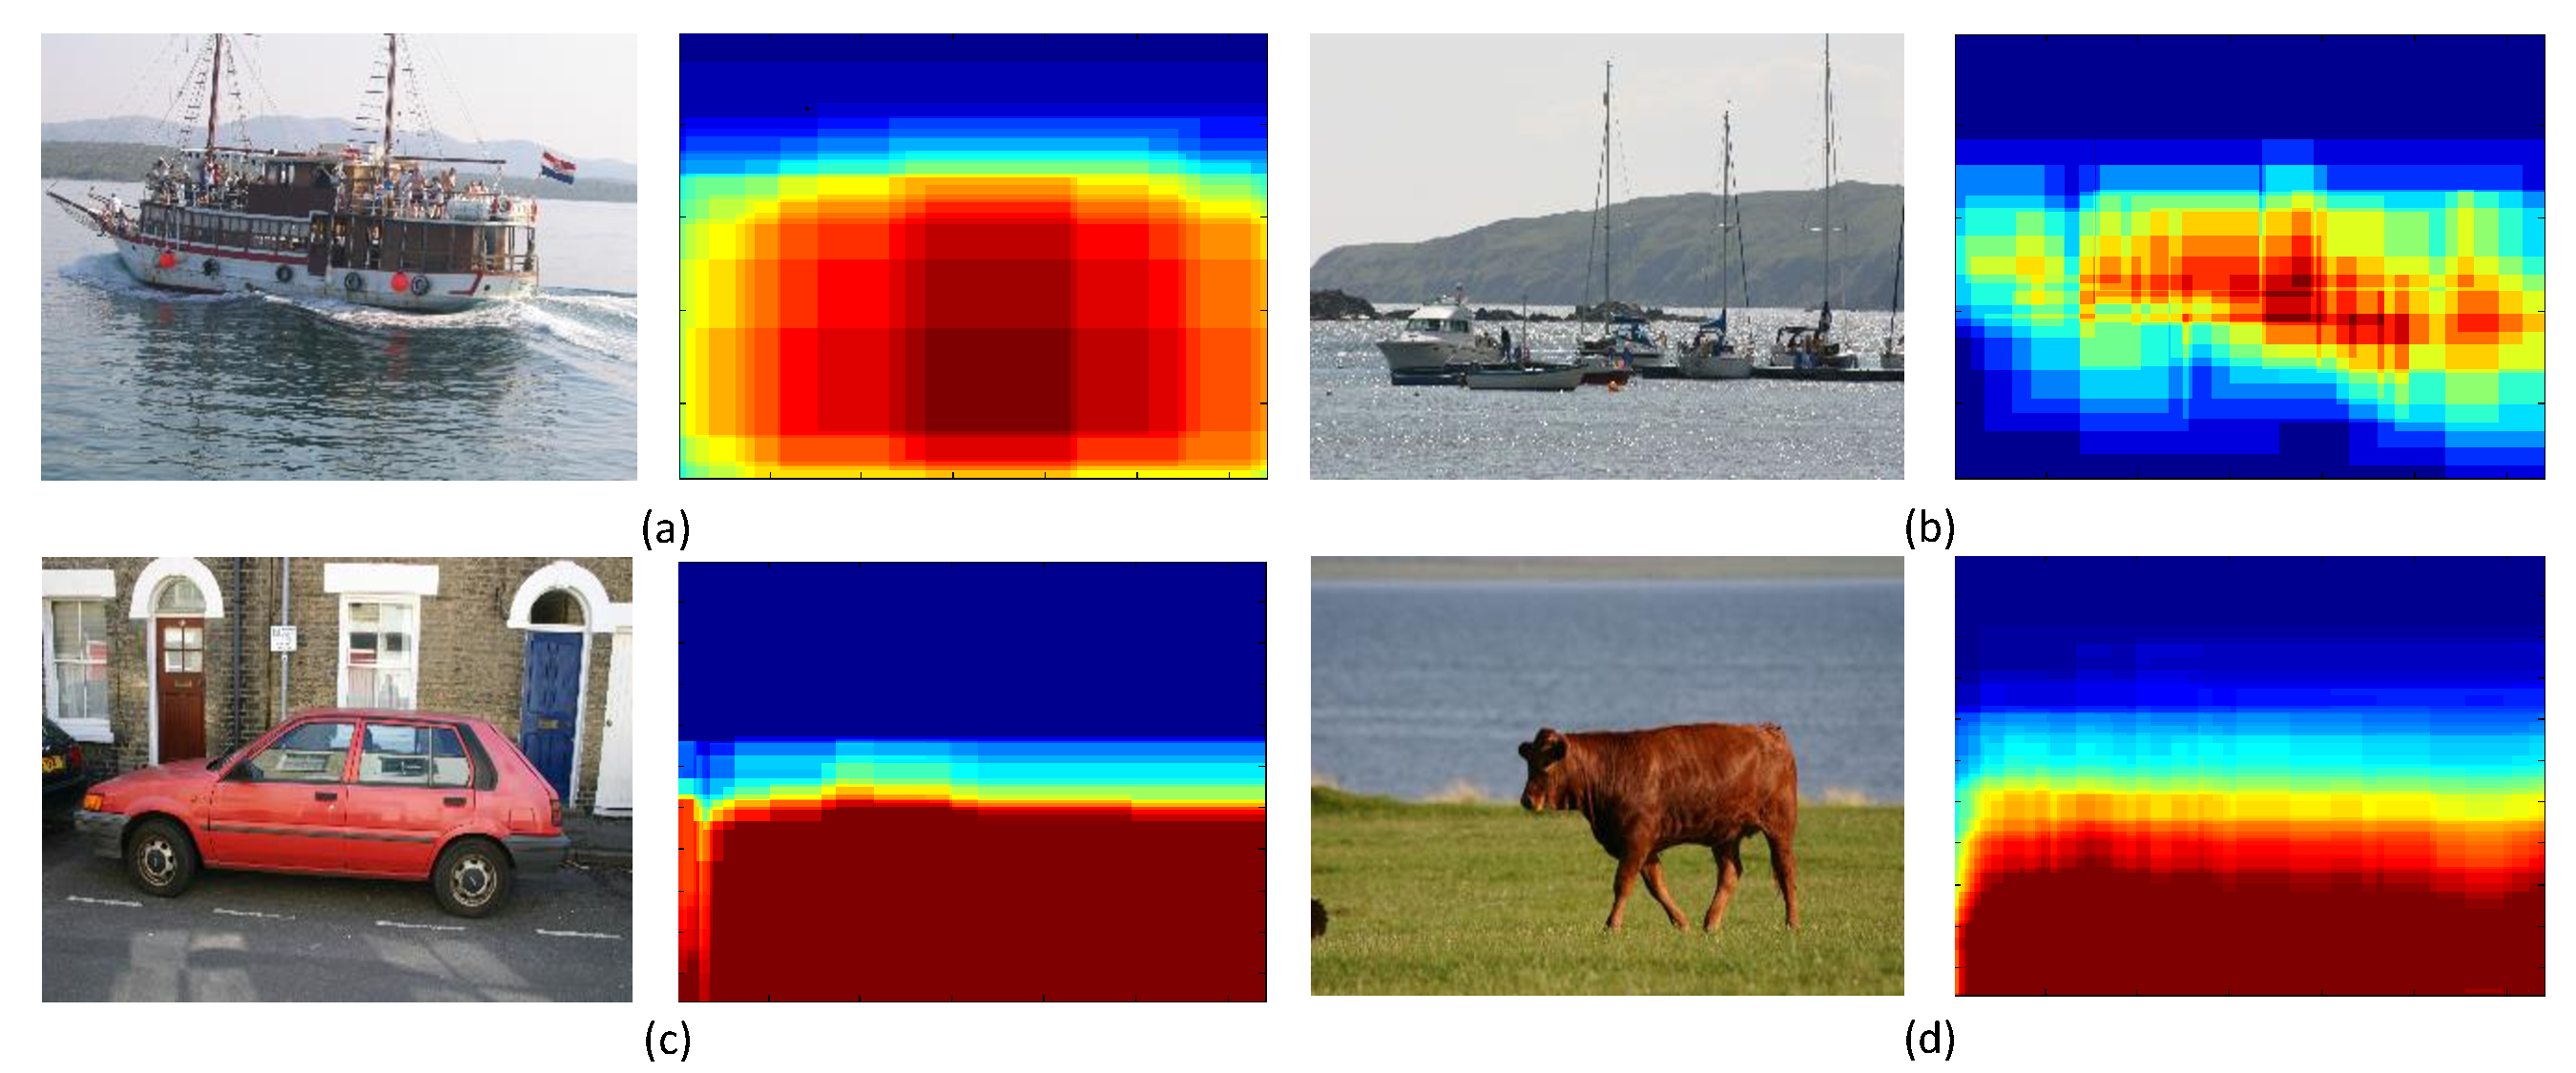
\includegraphics[width=0.6\linewidth]{figures/votemap.pdf}
\end{center}
\caption{Examples of our context vote maps. Each pair of images corresponds to the original image and the vote-based probability map of object location from observed context. From (a) - (d) are the vote maps from water to boat, sky to boat, road to car and grass to cow, respectively. Best viewed in color.}
\label{fig:votemap}
\end{figure}



The final context probabilistic vote map is given by
\begin{eqnarray}
p(c_t|c,X) = \sum_{s\in X^t} p(c_t|X_s)\sum_i W(s_{c_t}^i,s;\theta^W).T(b_{c_t}^i,b_c^i)\nonumber\\
\end{eqnarray}
where $p(c_t|X_s)$ is the probabilities of $s$ as class $c_t$ after taking the action $a_t$ to run classification at time $t$.


\section{Implementation Details}
\subsection{Object Proposals}
We use MCG object proposals in~\cite{arbelaez2014multiscale} as object candidates. Since the object proposals mainly covers the objects,  we also generate a small amount (20$\sim$30 per image) of segments using stable segmentation algorithm in~\cite{chen2011piecing} to cover the whole scene including contextual classes. To reduce the run-time retrieval overhead, our context voting step uses only the stable segments. The stable segmentation gives a coarse level of object/context division and can reduce the computation complexity of context voting compared to the large number of finer object proposals, while still maintains a semantically reasonable context inference. 

\subsection{Datasets}
We conduct our training and experiments on the Pascal VOC dataset.~\cite{Everingham10} which is a \textit{de facto} benchmark for object detection for years. Since the original dataset does not provide annotation of segmentation and contextual classes, we train our policy using the Pascal Context dataset~\cite{mottaghi2014role} which fully annotates the every pixels of the Pascal VOC 2010 train and validation sets, with additional contextual classes, which is perfectly good for our task. We use the 33 context classes and train our policy on the Pascal Context training set, and test our algorithm and baselines on the validation set. We also test our policy on the MSRC dataset~\cite{shotton2006textonboost} to show our algorithm can generalize to different data. 

